\chapter{Installation of Unitex}
\label{chap-install}

Unitex is a multi-platform system that runs on Windows as well as on Linux or
MacOS. This chapter describes how to install and how to launch Unitex on any of
these systems. It also presents the procedures used to add new languages and to
uninstall Unitex.

\section{Licenses}
\label{section-licences}
\index{LGPL}\index{License!LGPL}
Unitex is a free software. This means that the sources of the programs are
distributed with the software, and that anyone can modify and redistribute them.
The code of the Unitex programs is under the LGPL licence (\cite{LGPL}), except
for the TRE library for dealing with regular expressions from Ville Laurikari
(\cite{TRE}), which is under 2-clause BSD licence which is more
permissive than the LGPL. The LGPL Licence is more permissive than the GPL
licence, because it makes it possible to use LGPL code in nonfree software. 
From the point of view of the user, there is no difference,
because in both cases, the software can freely be used and distributed.

\bigskip
\noindent All the data that go with Unitex are distributed under the LGPLLR
license \index{LGPLLR} (\cite{LGPLLR}).

\bigskip
\noindent Full text versions of LGPL, 2-clause BSD and LGPLLR can be found in
the appendices of this manual.

\section{Java runtime environment}
Unitex consists of a graphical interface written in Java and external programs
written in \textit{C/C\kern-.05em\raisebox{.5ex}{++}\kern-.1em}. This mixture of
programming languages is responsible for a fast and portable application that
runs on different operating systems.

\bigskip
\noindent Before you can use the graphical interface, you first have to install the runtime
environment, usually called Java virtual machine \index{Java virtual machine} or
JRE\index{JRE} (Java Runtime Environment\index{Java Runtime Environment}).

\bigskip
\noindent For the graphical mode, Unitex needs Java version 1.6 (or newer). If you have an
older version of Java, Unitex will stop after you have chosen the working
language.

\bigskip
\noindent You can download the virtual machine for your operating system for free from the
Sun Microsystems web site (\cite{site-java}) at the following address:
\url{http://java.sun.com}.

\bigskip
\noindent If you are working under Linux or MacOS, or if you are using a Windows version
with personal user accounts, you have to ask your system administrator to install
Java.


\section{Installation on Windows}
\index{Installation!on Windows}
If Unitex is to be installed on a multi-user Windows machine, it is recommended
that the systems administrator performs the installation. If you are the only
user on your machine, you can perform the installation  yourself.

\bigskip
\noindent Decompress the file \index{File!\verb+Unitex3.0beta.zip+} \verb+Unitex3.0beta.zip+ (You
can download this file from the following address:
\url{http://www-igm.univ-mlv.fr/~unitex}) into a directory \verb+Unitex3.0beta+ that
should preferably be created within the \verb+Program Files+ folder.

\bigskip
\noindent After decompressing the file, the \verb+Unitex3.0beta+ directory contains several
subdirectories  one  of which is called \verb+App+. This directory contains a
file called \verb+Unitex.jar+. \index{File!\verb+Unitex.jar+} This file is the
Java executable that launches the graphical interface. You can double click on
this icon to start the program. To facilitate launching Unitex, you may want to
add a shortcut to this file on the desktop.




\section{Installation on Linux}
\index{Installation!on Linux}
In order to install Unitex on Linux, it is recommended to have system
administrator permissions. Uncompress the file \verb+Unitex3.0beta.zip+ in a
directory named \verb+Unitex+, by using the following command:

\bigskip \noindent \verb$unzip Unitex3.0beta.zip -d Unitex$

\bigskip
\noindent Within the directory \verb|Unitex/Src/C++/build|, start the compilation
of Unitex with the command:

\bigskip \verb+make install+

\bigskip
\noindent or with the following if you have a 64 bits computer:
 
\bigskip \verb+make install 64BITS=yes+

\bigskip
\noindent You can then create an alias in the following way:

\bigskip \verb$alias unitex='cd /..../Unitex/App/ ; java -jar Unitex.jar'$


\section{Installation on MacOS X}
\index{Installation!on MacOS X}
\label{section-macos-install}
\noindent NOTE: this short tutorial will tell you how to install and run 
Unitex on Mac OS X. Your questions, comments, suggestions, 
corrections are more than welcome. 

\noindent Contact: \url{cedrick.fairon@uclouvain.be}

\bigskip
\noindent There is an official Java 1.6 for MacOS X 10.5, 64-bit Intel 
(Core 2 Duo), but there is no official solution for older OS X (10.4 or older),
PowerPC and 32-bit Intel (Core Duo). So,
\begin{enumerate}
    \item if you have OS X 10.5, and 64-bit Intel MacOS, you can just get the
    Apple JRE 1.6. The only problem is that this version does not start by
    default. See section ``Java for Mac OS X 10.5 Update 2'', 
    at \url{http://developer.apple.com/java/}

    \item if you have an older OS X, 32-bit Intel or a PowerPC, you must try
    SoyLatte (see below)
\end{enumerate}

\noindent\textbf{How to know if my processor is a 32 or 64-bit one ?}

\noindent In the Apple menu, click on "About this Mac". If you see something
like: "Processor : x.xx Ghz Intel Core Duo", your processor is a 32-bit one.

\bigskip
\noindent If you see "Processor : x.xx Ghz Intel Core 2 Duo", or if you
processor is another Intel one (like Xeon), then you have a 64-bit processor.

\subsection{Using the Apple Java 1.6 runtime}
\bigskip\index{Using the Apple Java 1.6}
\noindent If you are running Mac OS X 10.5 (or later) on 64-Bits Intel processor, you can just use the Java 1.6 from Apple.\ You can get it from \url{http://www.apple.com/support/downloads/javaformacosx105update1.html}.

\noindent\ You can just start Application -> Utilities -> Java Preferences to verify the status of Java 1.6. First, be sure that "Java SE 6" is on "Java Applications" list
\begin{figure}[!h]
\begin{center}
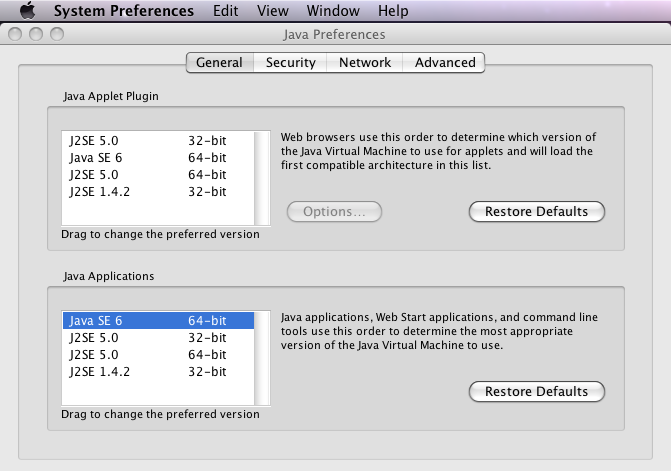
\includegraphics[width=13cm]{resources/img/java_pref_osx.png}
\caption{Checking and modify Java Preferences\label{fig-mac0}}
\end{center}
\end{figure}


\subsubsection{Option 1 : modify the default runtime for Java Applications}
\noindent If you don't use other Java application that need Java 1.5, you can just put "Java SE 6" at the top of the "Java Applications" list on Java Preference Utility.

\subsubsection{Option 2 : Create an alias to start Java 1.6}
\noindent If you don't want modify Java global parameters, you can create an
alias:

\bigskip
\noindent \verb+alias jre6="/System/Library/Frameworks/JavaVM.framework/Versions/+
\noindent \verb+1.6/Commands/java"+
   
\bigskip
\noindent \verb+jre6 -jar Unitex.jar+

\bigskip
\noindent Then just run Unitex from Terminal.

\subsection{SoyLatte}
\bigskip\index{SoyLatte}
\noindent SoyLatte is a functional, X11-based port of the FreeBSD
Java 1.6 patchset to Mac OS X Intel machines. SoyLatte is initially focused on 
supporting Java 6 development; however, the long-term view far more captivating: 
open development of Java 7 for Mac OS X, with a release available in concert 
with the official Sun release, supported on all recent versions of Mac OS X.

\subsubsection{Before you start}
\noindent Try it at your own risks ;-) This tutorial tells you what I have done
to have Unitex running on my MacBook Pro (Mac OS X 10.5.7), but it offers no guarantee 
that it will work  on your computer and it does not even guarantee that you can 
install it safely on your computer.

\bigskip
\noindent If you are not familiar with software installation, you should ask for
help. As Windows would put it ``Contact your Administrator'' ;-) 

\bigskip
\noindent It works only on Intel based Macintosh If you do not know whether your 
Macintosh is an Intel machine or not, select in the Apple Menu the item 
``About this Macintosh'', then, click on ``More info'' and in the next panel,
click on ``Hardware'', as shown on Figure \ref{fig-mac1}.

\begin{figure}[!h]
\begin{center}
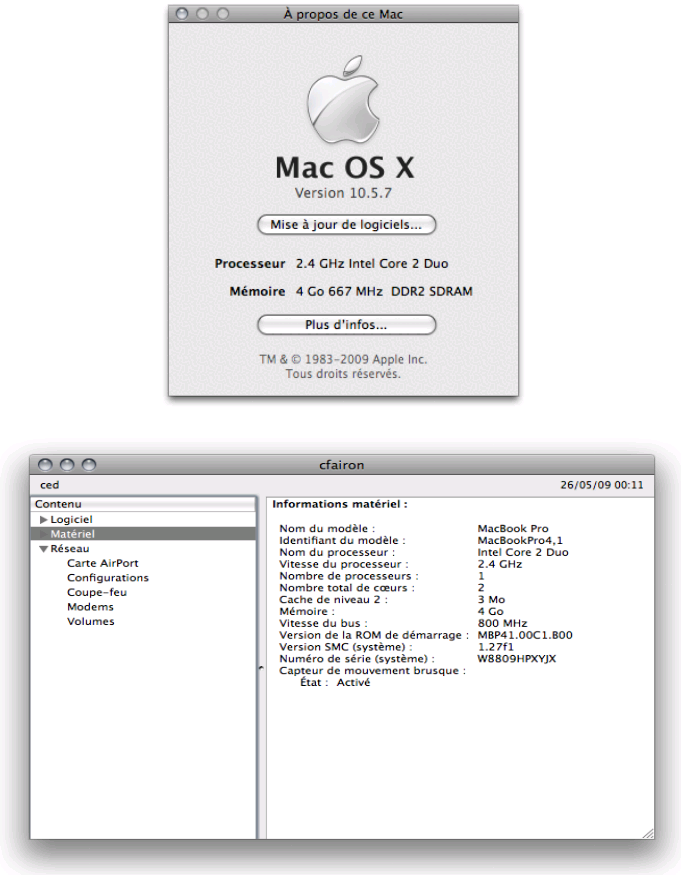
\includegraphics[width=13cm]{resources/img/fig-mac1.png}
\caption{Getting information on your computer\label{fig-mac1}}
\end{center}
\end{figure}

\clearpage

\subsubsection{Installation}
\noindent Some of the following installation steps will require the use of the
terminal application. On MacOS, the terminal application is located in 
\verb+/Applications/Utilities/Terminal.app+.  When you start this application
(double click) a window is displayed. You will have to type in this window 
some commands for moving, editing and installing files.

\subsubsection{Install X11.app}
\index{X11.app}
\noindent X11 is available as an optional install on the Mac OS X v10.3 
Panther, and Mac OS X v10.4 Tiger install disks (the disks you received 
when you bought your computer). Run the Installer, 
select the X11 option, and follow the instructions.

\bigskip
\noindent After installation X11 will be available in
\verb+/Applications/Utilities/+


\subsubsection{Download and install Unitex as usual}
\noindent Download Unitex and uncompress it in the same way that for Linux.
See section \ref{section-mac-compilation} for instructions on compiling
C++ programs.


\subsubsection{Download SoyLatte (the Java 1.6 port)} 
\noindent It is available from
\url{http://landonf.bikemonkey.org/static/soylatte/} 

\bigskip
\noindent Unless you know why you need another package, you will chose 
the 32-Bit Binaries distribution (32-bit JDK for Mac OS X 10.4 and 10.5) 
When prompted, enter the username and password: 

\bigskip
Username: \verb+jrl+

Password: \verb+I am a Licensee in good standing+


\subsubsection{Install SoyLatte}
\noindent Either in command line mode:
\begin{itemize}
    \item Open the terminal (\verb+/Applications/Utilities/Terminal+)
    \item Find the SoyLatte archive. If it is on your desktop, change the
    current directory by typing the following command in the terminal 
    (the character \verb+~+ means 'home directory'): 
    
    \bigskip
    \verb+cd ~/Desktop/+
    
    \item Move (\verb+mv+) the archive anywhere on your file system (where you
    want to install it). If you chose \verb+/usr/local+, like me, it requires the
    administrative privileges (use \verb+sudo+ and type your password when
    prompted). Note, if the directory does not exist, you can create it 
    before you move the file:
    
    \bigskip
    \verb+sudo mkdir /usr/local         + (only if it does not exist)
    
    \verb+sudo mv soylatte16-i386-1.0.3.tar.bz2 /usr/local/+

    \item Uncompress the archive:
    
    \bigskip
    \verb+sudo tar -jxvf /usr/local/soylatte16-i386-1.0.3.tar.bz2+ 
\end{itemize}

\bigskip
\noindent or, using the graphical interface (finder):
\begin{itemize}
    \item Move (drag and drop) the archive
    
    %do not remove this line jump
    \noindent \verb+soylatte16-i386-1.0.3.tar.bz2+ into the \verb+/Applications+ folder
    \item Double-click on it... wait... it's done ;-)
\end{itemize}


\subsubsection{Configure your system}
\noindent There are two approaches: you could either decide to use SoyLatte only
with Unitex (and keep using the former version of Java that is already installed 
on your computer for all the others Java applications) or decide to make SoyLatte 
the default Java distribution on your machine.

\bigskip
\noindent As I have no indication that SoyLatte is bug free and fully
functional with all applications, I chose to use SoyLatte only with 
Unitex and kept my Java (and I recommend the same for you). If you 
want to follow this advice: DO NOT modify your PATH variable as suggested 
in the SoyLatte installation procedure. Instead add an ALIAS in the configuration 
file of your shell. Here is how to do that:
\begin{itemize}
    \item Edit the bash configuration file, which is in your home directory 
    (\verb+/Users/your_dir_name+); The easiest way to do it is to use a command
    line editor like \verb+vim+ or \verb+pico+ (note: \verb+.bashrc+ is a hidden
    file. So, normally, you will not see this file in the Finder):
    
    \bigskip
    \verb+pico ~/.bashrc+
    
    \item In the file, type the following lines :
    
    \bigskip
    \verb+alias java6='/usr/local/soylatte16-i386-1.0.3/bin/java'+
    
    \verb+alias unitex='cd /Applications/Unitex3.0beta/App ; java6 -jar+
    
    \verb+Unitex.jar'+
    
    \bigskip
    \noindent The first line creates and alias that makes it easy to run
    SoyLatte-Java and the second line creates and alias that makes it easy to start Unitex.
    
    \item Then, quit \verb+pico+ (type CTRL+x, answer ``yes'' to the question
    ``Do you want to save?'' and then press Enter to proceed).
\end{itemize}

\noindent Changes will be active next time the \verb+.bashrc+ file is loaded
(quit and re-launch \verb+Terminal.app+ or more simply, type \verb+bash+ to open
a new bash session). Once you have a new bash session, type the command 
\verb+unitex+ and let's start using Unitex on your Mac !!

\begin{figure}[!h]
\begin{center}
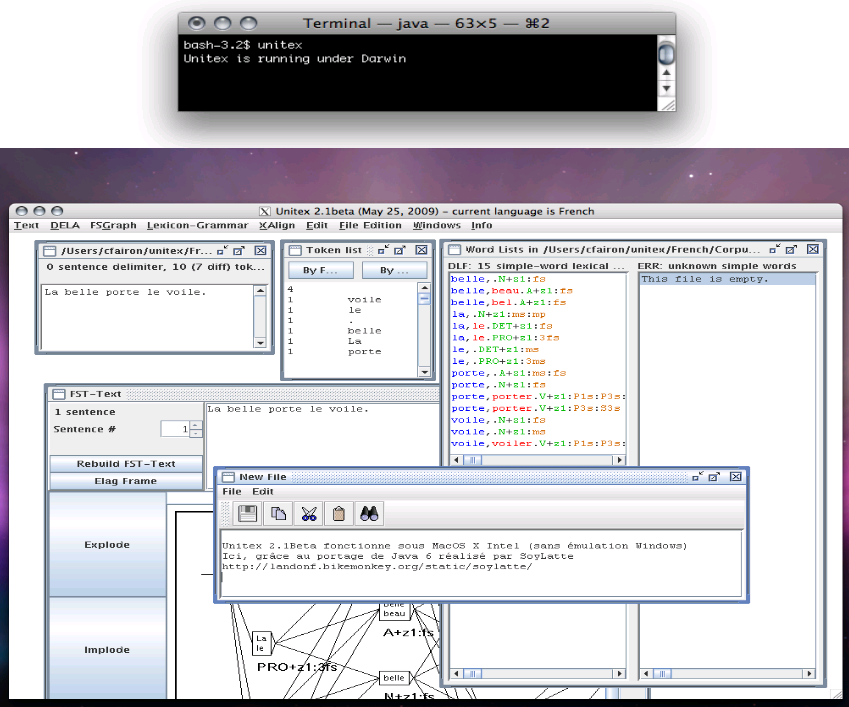
\includegraphics[width=13cm]{resources/img/fig-mac2.png}
\caption{Running Unitex on Mac\label{fig-mac2}}
\end{center}
\end{figure}

\subsection{How to compile Unitex C++ programs on a Macintosh}
\label{section-mac-compilation}
\noindent In order to install Unitex on Mac OS, you will have to compile
Unitex C++ sources. This is not a problem if you have already the common 
(\verb+gcc+) development tools installed on your computer (but of course, they
are not in the standard installation).

\bigskip
\noindent If you don't know if these tools are present, don't think too long
about it... just give a try; open a shell window, move to the Unitex sources
directory (\verb$cd /path/to/Src/C++/build$) and run the command that starts the
compilation: \verb+make install+

\begin{figure}[!h]
\begin{center}
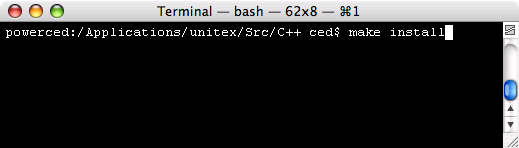
\includegraphics[width=12cm]{resources/img/fig-mac3.png}
\caption{Compiling Unitex C++ programs\label{fig-mac3}}
\end{center}
\end{figure}

\bigskip
\noindent If the compilation does not start and you get an error message
stating that the command \verb+make+ cannot be found, you probably need to
install development programs. On Macintosh the ``all inclusive development
bundel'' is ``Xcode'' \index{Xcode}(current version is 2.2 and it includes a lot
of stuff among which). Your can donwload it from the Apple developer Web site.

\bigskip
\noindent The Xcode application includes a full-featured code editor, a debugger, 
compilers, and a linker. The Xcode application provides a user interface to many 
industry-standard and open-source tools, including \verb+gcc+, the Java compilers
\verb+javac+ and \verb+jikes+, and \verb+gdb+. It provides all of the facilities you
need to build a program for Mac OS X, whether it's an application, kernel
extension, or command-line tool.

\bigskip
\noindent The only problem with Xcode is that it is HUGE to download (800 Mb).
Of course, you will not need all the stuff included in the package... but all
what you need is in it.

\begin{figure}[!h]
\begin{center}
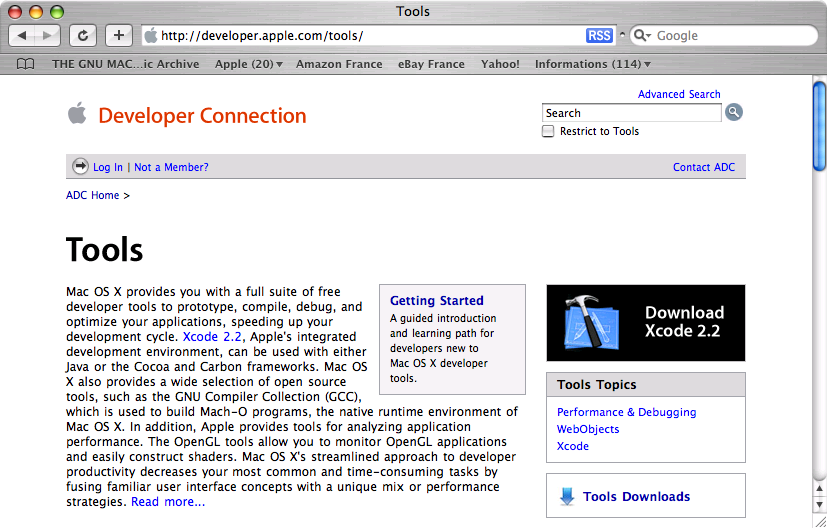
\includegraphics[width=15cm]{resources/img/fig-mac4.png}
\caption{Xcode\label{fig-mac4}}
\end{center}
\end{figure}


\bigskip
\noindent Once on your computer the Xcode package looks like the following:

\begin{figure}[!h]
\begin{center}
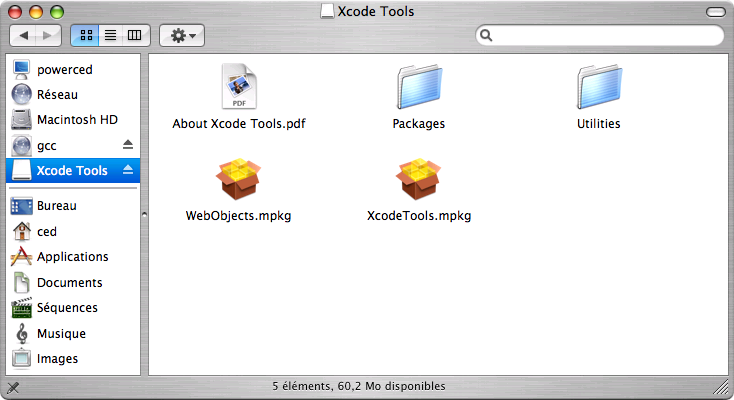
\includegraphics[width=14cm]{resources/img/fig-mac5.png}
\caption{Xcode package\label{fig-mac5}}
\end{center}
\end{figure}


\bigskip
\noindent Double-click on the \verb+XCodeTools.mpkg+ icon to install all the
programs.


\subsection{How to makes all files visible on Mac OS}
\noindent See
\url{http://www.macworld.com/article/51830/2006/07/showallfinder.html}.

\bigskip
\noindent Or try it right away... Type: 

\bigskip
\verb+defaults write com.apple.Finder AppleShowAllFiles ON+

\bigskip
\noindent Then restart the Finder:

\bigskip
\verb+killall Finder+

\begin{figure}[!h]
\begin{center}
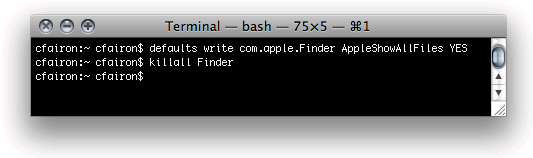
\includegraphics[width=12cm]{resources/img/fig-mac6.png}
\caption{Restarting the Finder\label{fig-mac6}}
\end{center}
\end{figure}

\bigskip
\noindent To get back to the original configuration, type: 

\bigskip
\verb+defaults write com.apple.Finder AppleShowAllFiles OFF+


\section{First use}
If you are working on Windows, the program will ask you to choose a
\index{Directory!personal working} personal working  directory, which you can
change later in "Info>Preferences...>Directories". To create a directory, click
on the icon showing a file (see
figure~\ref{fig-creation-personal-directory}).

\bigskip
\noindent If you are using Linux or MacOS, the program will automatically create a
\verb+/unitex+ directory in your \verb+$HOME+ directory. This directory allows
you to save your personal data. For each language that you will be using, the
program will copy the root directory of that language to your personal
directory, except the dictionaries. You can then modify your copy of the
files without risking to damage the system files.

\begin{figure}[h]
\begin{center}
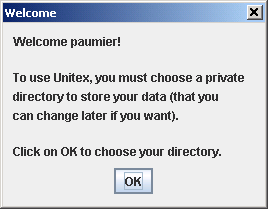
\includegraphics[width=6.3cm]{resources/img/fig1-1.png}
\caption{First use under Windows}
\end{center}
\end{figure}

\begin{figure}[h]
\begin{center}
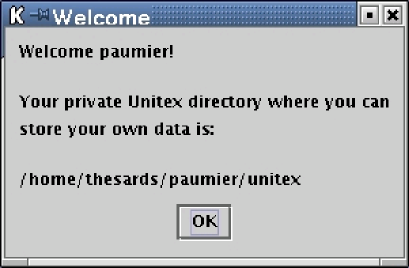
\includegraphics[width=7cm]{resources/img/fig1-2.png}
\caption{First use under Linux}
\end{center}
\end{figure}

\begin{figure}[h]
\begin{center}
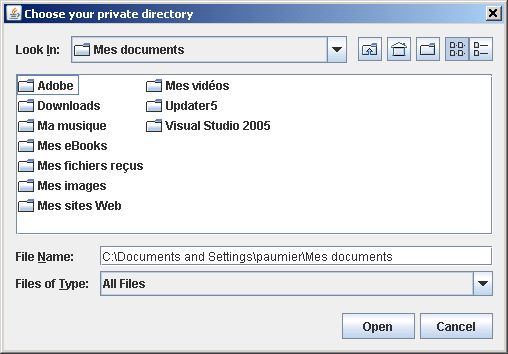
\includegraphics[width=13cm]{resources/img/fig1-3.png}
\caption{Creating the personal work
directory\label{fig-creation-personal-directory}}
\end{center}
\end{figure}



\section{Adding new languages}
\index{Adding languages}

\bigskip
\noindent There are two different ways to add languages. If you want to add 
a language that is to be accessible by all  users, you have to copy the 
corresponding directory to the \verb+Unitex+ system directory, for which 
you will need to have the access rights  (this might mean that you need to 
ask your system administrator to do it). On the other hand, if the language 
is only used by a single user, he can also copy the directory to his working 
directory. He can work with this language without this language being shown to other users.


\section{Uninstalling Unitex}
No matter which operating system you are working with, it is sufficient to delete 
the \verb+Unitex+ directory to completely delete all the program files. Under
Windows you may have to delete the shortcut to \verb+Unitex.jar+ \index{File!\verb+Unitex.jar+} 
if you have created one on your desktop. The same has to be done on Linux, if you have 
created an alias.


\section{Unitex for developpers}
\label{section-unitex-developpers}
If you are a programmer, you may be interested in linking your code with Unitex
C++ sources. To facilitate such operation, you can compile Unitex as a
dynamic library that contains all Unitex functions, except \verb+main+s, of
course. Under Linux/MacOS, type:

\bigskip
\verb+make LIBRARY=yes+

\bigskip
\noindent and you will obtain a library named \verb+libunitex.so+. If you want
to produce a Windows DLL named \verb+unitex.dll+, use the following commands:

\bigskip
Windows: \verb+make SYSTEM=windows LIBRARY=yes+

Cross-compiling with mingw32: \verb+make SYSTEM=mingw32 LIBRARY=yes+

\bigskip
\noindent In all cases, you will also obtain a program named
\verb+Test_lib+(\verb+.exe+). If everything worked fine, this program should 
display the following:

\begin{verbatim}
Expression converted.
Reg2Grf exit code: 0

#Unigraph
SIZE 1313 950
FONT Times New Roman:  12
OFONT Times New Roman:B 12
BCOLOR 16777215
FCOLOR 0
ACOLOR 12632256
SCOLOR 16711680
CCOLOR 255
DBOXES y
DFRAME y
DDATE y
DFILE y
DDIR y
DRIG n
DRST n
FITS 100
PORIENT L
#
7
"<E>" 100 100 1 5
"" 100 100 0
"a" 100 100 1 6
"b" 100 100 1 4
"c" 100 100 1 6
"<E>" 100 100 2 2 3
"<E>" 100 100 1 1
\end{verbatim}
